\section{Laboratory work implementation}

\subsection{Tasks and Points}
\begin{itemize}
\item \textbf{Basic Level (grade 5 - 6) you should be able to:}
	\begin{enumerate}
	\item Draw 5 lines of different colors and weights
      \item Draw 2 Bezier curves
      \item Draw 4 plane objects (ex. circle, square, pie, polygon...) of different colors, weights, filled and not
      \item Draw 2 different objects using mouse
      \end{enumerate}
\item \textbf{Normal Level (grade 7 - 8) you should be able to:}
      \begin{enumerate}
    \item Realize the tasks from \textit{Basic Level}.
    \item Draw a custom bitmap image
    \item Fill object with gradient
    \item Hook keyboard input. Add 2 different keyboard combinations that will change mouse ability to draw objects (ex. on Ctrl+C will draw circles, on Alt+R will continue to draw circles but of read color)
    \item Draw a Bezier curve using mouse
          \end{enumerate}
\item \textbf{Advanced Level (grade 9 - 10) you should be able to:}
      \begin{enumerate}
    \item Realize the tasks from \textit{Normal Level}.
    \item use mouse as an eraser (choose 1 option):
    	\begin{enumerate}
        \item eraser of a fixed width
        \item delete objects using mouse clicking
        \item eraser with adjustable width
        \end{enumerate}
          \end{enumerate}
\item \textbf{for Bonus Point Tasks :}
\begin{enumerate}
	\item Realize the task with mouse eraser for all 3 cases listed above. In order to choose one of them, add 3 buttons/icons or check boxes.
    \end{enumerate}
  \end{itemize}  

\clearpage
\subsection{Prove your work with screens}



\begin{figure}[h!]
  \centering
    {%
      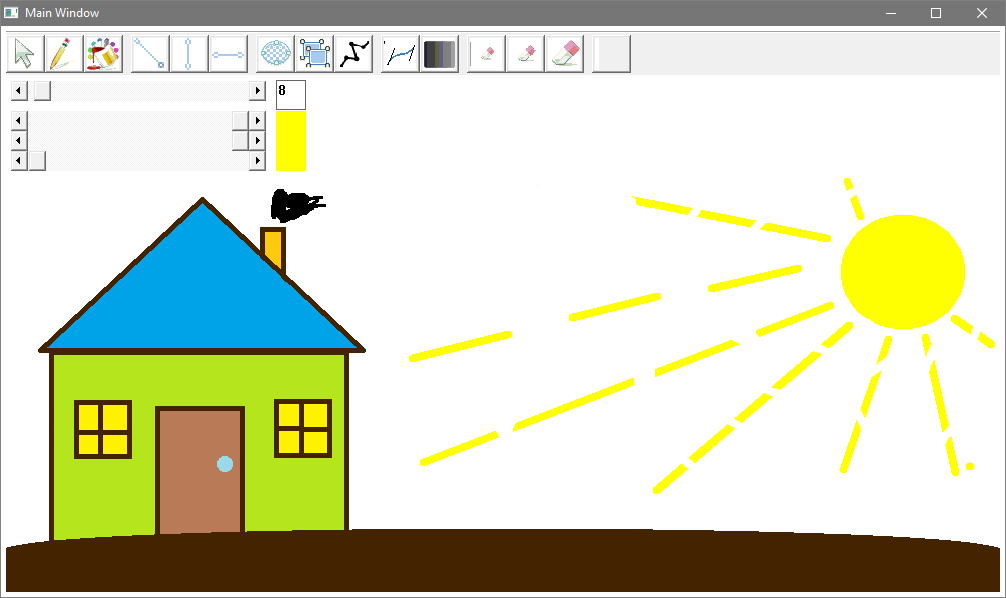
\includegraphics[width=1\textwidth]{3}}
  \caption{This is MaxPaint program that allows you to do something like this}
\end{figure}

\begin{figure}[h!]
  \centering
    {%
      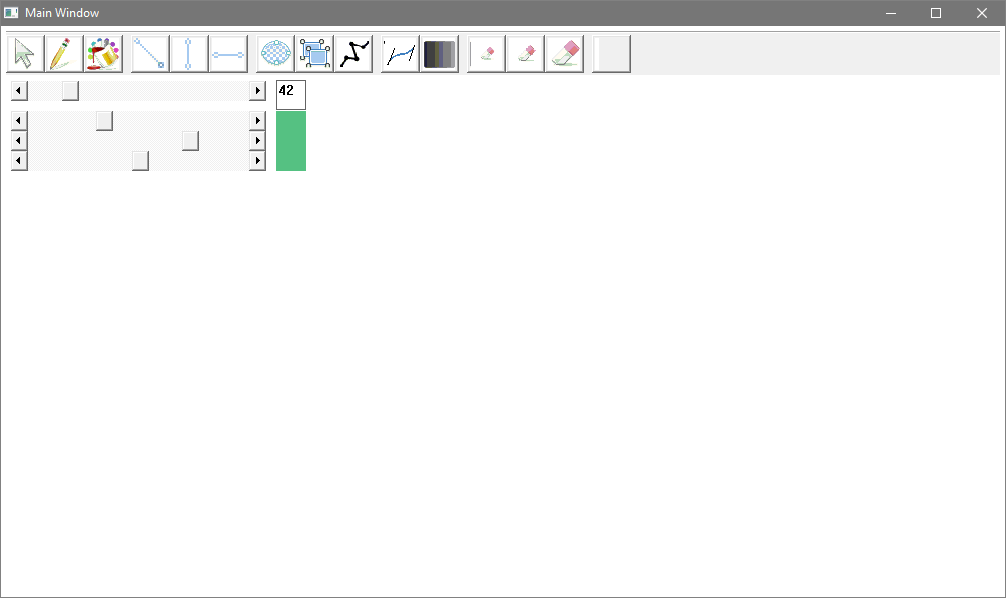
\includegraphics[width=1\textwidth]{1}}
  \caption{When user opens for the first time MaxPaint He will see something like this.}
\end{figure}

\begin{figure}[h!]
  \centering
    {%
      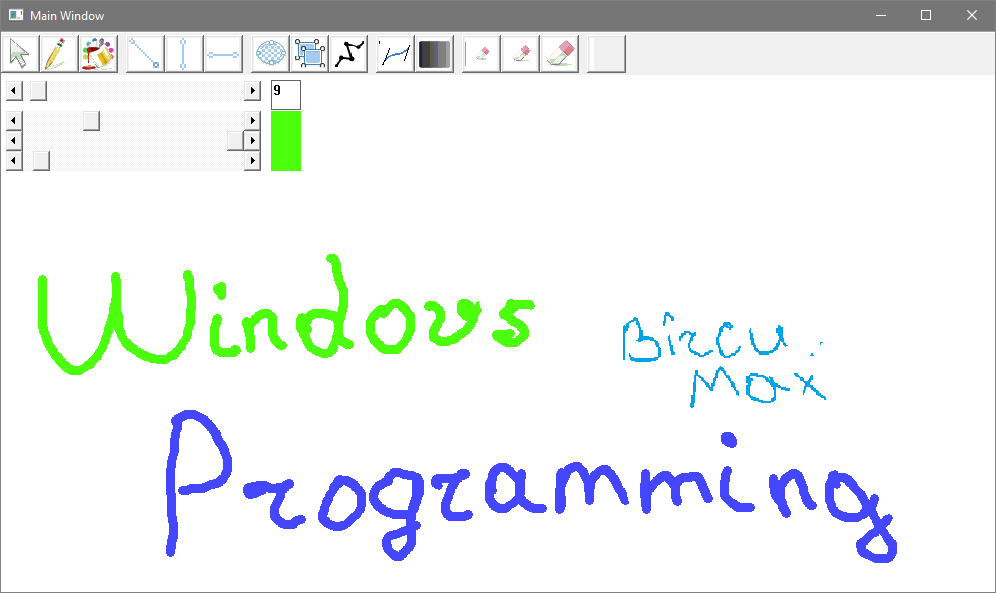
\includegraphics[width=1\textwidth]{6}}
  \caption{Chose pen tool from the program toolbar to draw free form lines, and also you can change the color and thickness of the pen by moving scrolls under the toolbar the first one is for thickness and the next 3 are for colors acording to R G B principle.}
\end{figure}

  
\begin{figure}[h!]
  \centering
    {%
      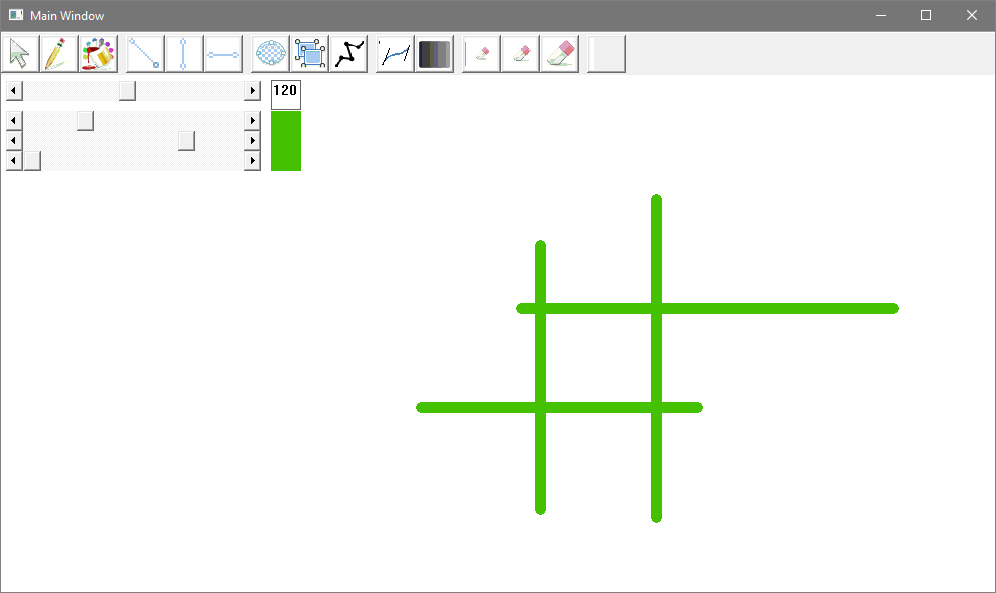
\includegraphics[width=1\textwidth]{5}}
  \caption{Also you can draw vertical or horizontal lines if you chose such tool form tool bar and again you can adjust thickness and color of drawing using scrolls under the toolbar}
\end{figure}


\begin{figure}[h!]
  \centering
    {%
      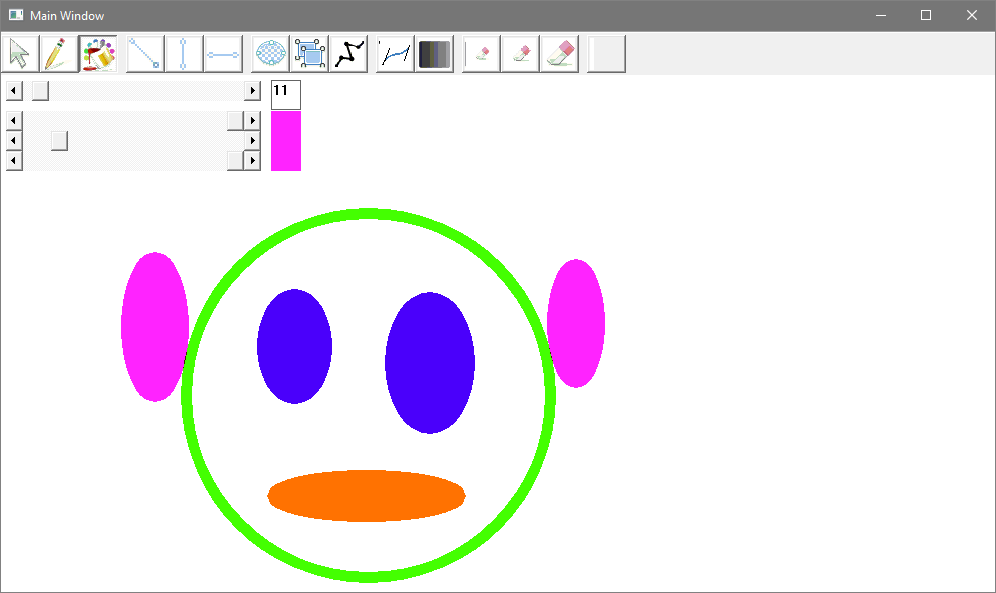
\includegraphics[width=1\textwidth]{8}}
  \caption{The next tool that I want to mention allows you to draw ellipses of different colors and thickness , also you can press CTRL+R for drawing regular objects in the case of ellipse they will be circles, also you can draw ellipse that are fill with a color. And again you can adjust colors and thickness from scrolls under the toolbar }
\end{figure}


\begin{figure}[h!]
  \centering
    {%
      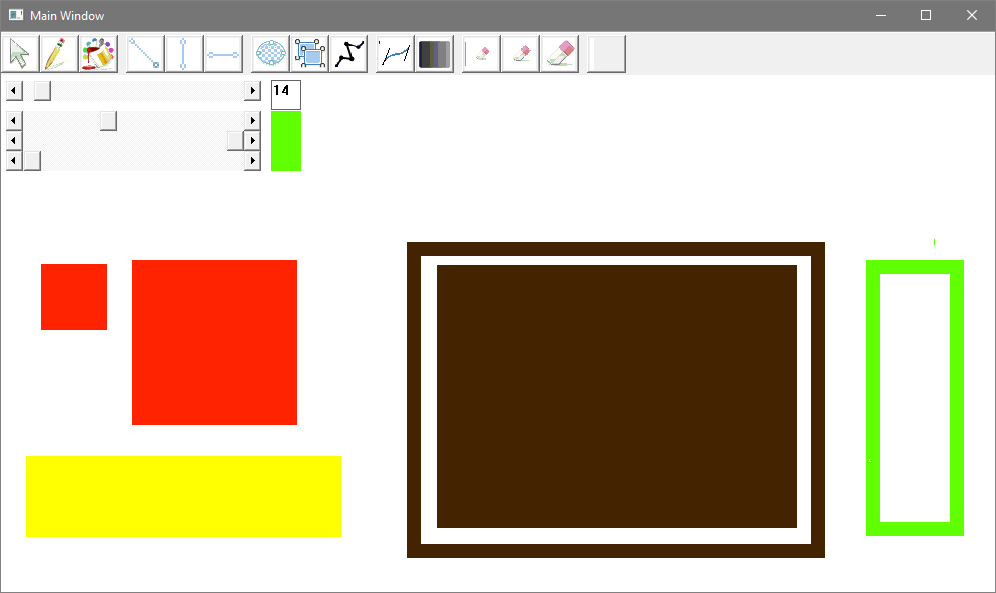
\includegraphics[width=1\textwidth]{9}}
  \caption{Another button from toolbar allows you to draw different tettragons, which color and thickness you can again change from scrolls under the toolbar. Also you can press CTRL-R to activate regular drawing to draw squares}
\end{figure}

\begin{figure}[h!]
  \centering
    {%
      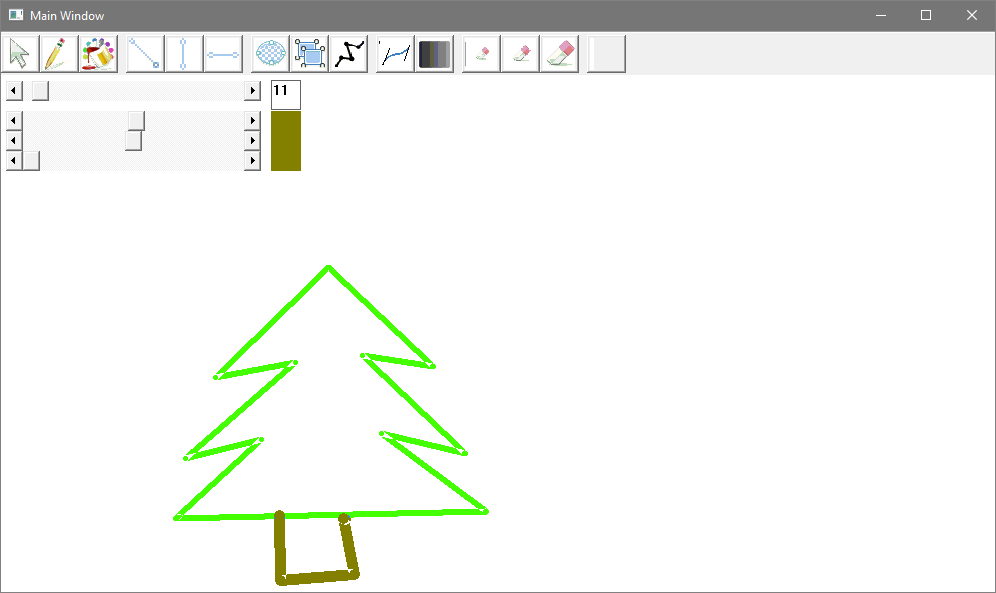
\includegraphics[width=1\textwidth]{10}}
  \caption{You can also draw poly lines or in other word connected lines by choosing the poly-line button from toolbar to exit from drawing you should press CTRL-E , and again you can change thickness and color from control scrolls  }
\end{figure}

\begin{figure}[h!]
  \centering
    {%
      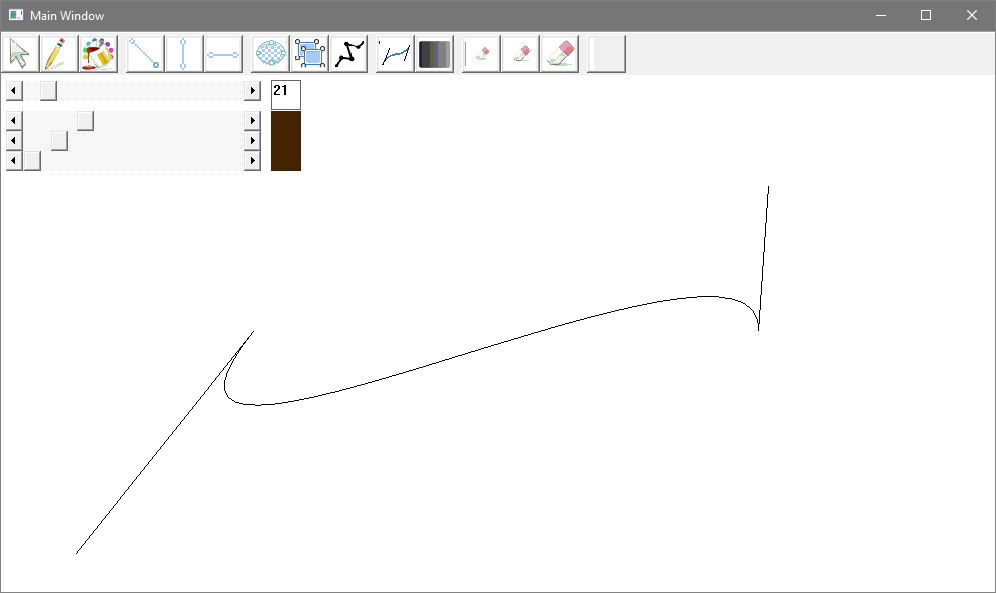
\includegraphics[width=1\textwidth]{11}}
  \caption{You can press bezier button and draw bezier, To modify the curve press left mouse button and drag and also you can press right mouse button and drag}
\end{figure}


\begin{figure}[h!]
  \centering
    {%
      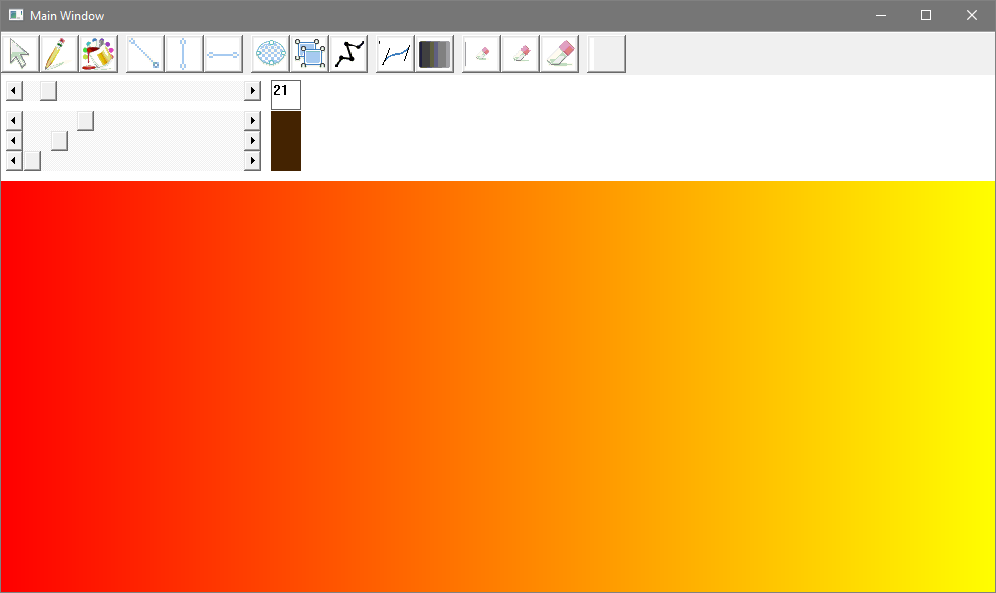
\includegraphics[width=1\textwidth]{14}}
  \caption{Press gradient button to fill the entire window with a predefined gradient color. }
\end{figure}

\begin{figure}[h!]
  \centering
    {%
      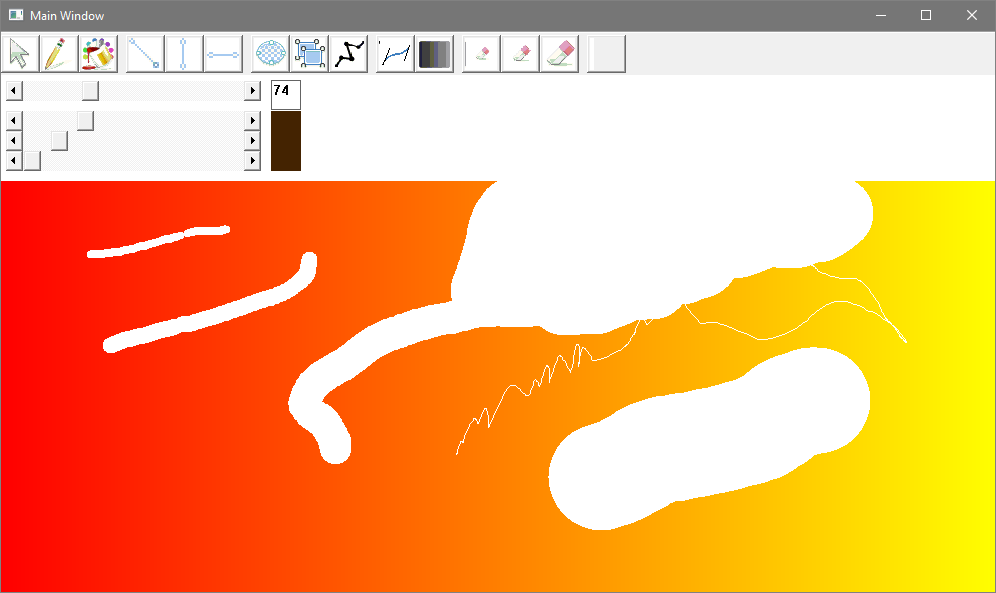
\includegraphics[width=1\textwidth]{15}}
  \caption{If you have drawn something wrong you can choose eraser button to erase , There are 3 eraser buttons off different sizes and one eraser button with adjustable size that can be adjusted from the thickens scroll controller.}
\end{figure}
